\documentclass[11pt, a4paper]{article}
\usepackage{ae, lmodern}
\usepackage[french]{babel}
\usepackage[utf8]{inputenc}
\usepackage[T1]{fontenc}
\usepackage{polytechnique}
\usepackage{amsmath}
\usepackage{amssymb}
\usepackage{amsfonts}
\usepackage{graphicx}


\author{Emeric \textsc{AURIANT} \\ Mathéo \textsc{VERGNOLLE}}
\title{INF421 - Projet de programmation}
\date{Février 2021}

\begin{document}
	
\maketitle

\begin{abstract}
	
L'objectif de ce sujet est de résoudre le problème du Rikudo, un jeu de logique populaire consitant à trouver un chemin dans une grille hexagonale. Pour cela nous utilisons deux algorithmes différents (SAT et Backtracking) et de générer aléatoirement des Rikudos en partant d'images bicolores. 

Résoudre un Rikudo correspond à résoudre un problème de chemin hamiltonien dans un graphe avec quelques contraintes supplémentaires. La première étape a donc été de définir des structures de données adaptées, puis de résoudre le problème des chemins hamiltoniens. Enfin de rajouter les contraintes du Rikudo, c'est à dire les labels et les diamants.

Pour générer un Rikudo à partir d'une image bicolore il faut d'abord savoir transformer un graphe en Rikudo et savoir obtenir un graphe à partir d'une image bicolore. 

\end{abstract}

\section{Structures de données utilisées}

Nous avons choisi de représenter un graphe ($\mathtt{Graph}$) par un tableau de listes d'adjacences, car dans un Rikudo chaque sommet a au plus six voisins. Les graphes considérés dans ce problème sont donc plutôt creux. Une représentation par matrice d'adjacence occuperait trop d'espace et augmenterait le temps de parcours des voisins.

Nous avons pour cela implémenté notre propre structure de liste chaînée simple ($\mathtt{intList}$, basée sur la version statique $\mathtt{Node.java}$). Cette version statique contient précisément les méthodes dont nous avions besoin et garantit notamment l'unicité et l'ordre de ses éléments.

\section{Chemin hamiltonien}

La première tâche était de trouver un chemin Hamiltonien dans un graphe, c'est à dire un chemin passant exactement une seule fois par chaque sommet. Nous avons pour cela utilisé deux stratégies, ainsi que l'indiquait le sujet : réduire notre problème à un problème SAT et le résoudre avec un solver SAT ($\mathtt{HamiltonianSAT}$), ou trouver un chemin avec un algorithme de Backtracking ($\mathtt{HamiltonianBT}$).

\subsection{Avec un solveur SAT}

\label{hamSAT}

Un problème SAT consiste à déterminer si une formule booléenne en Forme normale Conjonctive (conjonction de disjonction de littéraux) est satisfiable. Ce problème est NP-Complet. On implémente ici une réduction de notre problème au problème SAT et nous allons le résoudre avec un solveur de SAT dans la classe $\mathtt{HamiltonianSAT}$.

Trouver un chemin Hamiltonien revient à trouver une bijection entre les sommets (dans $[0, n- 1]$) et des labels (dans $[1, n]$). Suivant les indications de l'énoncé, nous avons considéré les variables booléennes $x_{i, v}$, valant $\mathtt{True}$ si et seulement si le sommet $v$ a le label $1$. Il faut alors ajouter des clauses correspondant aux contraintes du chemin hamiltonien :
\begin{enumerate}
	\item chaque sommet $v$ apparaît exactement une fois dans le chemin : pour tout $v$ dans $[0, n-1]$, exactement une des variables $\{x_{i, v}, i\in[1, n] \}$ est vraie
	\item chaque label $i$ est utilisé exactement une fois : pour tout $i$ dans $[1, n]$, exactement une des variables $\{x_{i, v}, v\in[0, n-1] \}$ est vraie
	\item des sommets consécutifs du chemin doivent être adjacents dans le graphe : pour tous $v, w$ sommets du graphes, s'il n'y a pas d'arête entre $v$ et $w$ alors on ne peut pas avoir $x_{i, v}$ et $x_{i+1, w}$ pour $i \in [1, n-1]$, i.e.
	\[\forall (v, w) \in E^C, \forall i \in [1, n- 1], \neg x_{i, v} \lor \neg x_{i+1, w}\]
	\item le chemin commence par la source et finit par la cible : $x_{1, s}$ et $x_{n, t}$ sont vraies
\end{enumerate}

On utilise la librairie $\mathtt{sat4j}$ pour résoudre ce problème SAT. Les contraintes 1 et 2 sont données au Solver en utilisant $\mathtt{org.sat4j.specs.ISolver.addExactly}$, les contraintes 3 et 4 en utilisant $\mathtt{org.sat4j.specs.ISolver.addClause}$. On peut ensuite reconstruire le chemin à partir de la solution renvoyée par le Solver.

La bibliothèque $\mathtt{sat4j}$ est utilisée comme une boîte noire, on ne peut pas évaluer sa complexité. On peut néanmoins remarquer que le nombre de clauses à satisfaire croît avec le nombre de paires de sommets qui \textbf{ne sont pas} reliés par une arête. On peut donc conjecturer que cette méthode sera plus efficace sur des graphes denses.

\subsection{Avec un algorithme de Backtracking}

On cherche maintenant à résoudre le problème des chemins hamiltoniens avec un algorithme de rebroussement ("backtracking"). L'algorithme se trouve dans la classe $\mathtt{HamiltonianBT}$. 

L'algorithme a plusieurs étapes. 

\begin{enumerate}
    \item On commence sur le sommet source.
    \item On ajoute  au chemin un sommet non visité et voisin du sommet actuel.
    \item Si le chemin peut-être complété en un chemin hamiltonien, on continue, sinon on enlève ce sommet du chemin et l'on revient à l'étape 2.
\end{enumerate}  

On arrête l'algorithme lorsque l'on trouve un chemin hamiltonien, c'est à dire lorsque le sommet actuel est le sommet target et que nous avons visité exactement une fois chaque sommet, pour cela on garde en mémoire le nombre de sommet visité et les sommets visités.

On cherche ensuite à compter le nombre de chemins hamiltoniens. L'algorithme n'est pas beaucoup plus compliqué. L'algorithme ne s'arrête pas lorsqu'on trouve un chemin. À la place, on incrémente un compteur et on rebrousse chemin (on supprime le dernier sommet du chemin et on continue). 

La complexité temporelle du premier algorithme est compliquée à estimer, mais nous savons qu'elle est majorée par celle du deuxième algorithme. Le deuxième algorithme parcourt tout les chemins du graphe, sa complexité temporelle est donc dominée par le nombre de chemins partant de la source dans le graphe. L'algorithme est donc efficace lorsque le nombre de chemin est faible, c'est à dire lorsque le graphe est creux.

\begin{figure}[h]
	\centering
	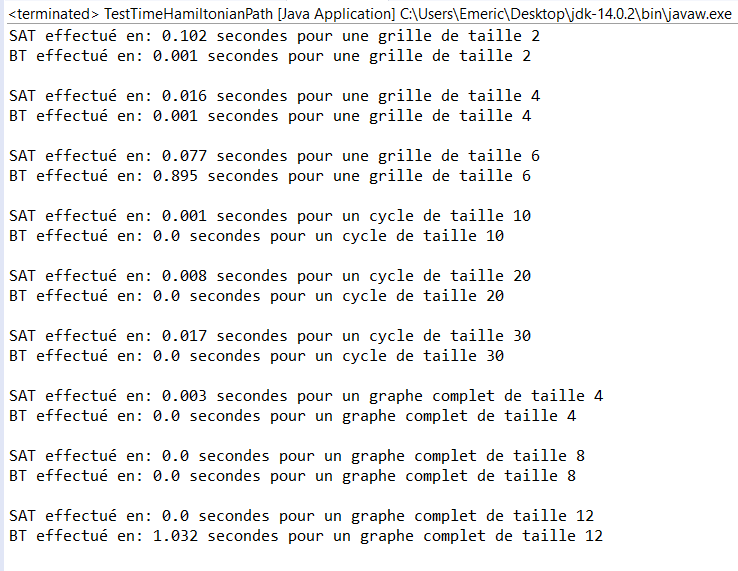
\includegraphics[scale=0.8]{RunTimeHamiltonianPath.png}
\end{figure}

\section{Ajout de contraintes}

La résolution d'un Rikudo peut-être considérée comme la recherche d'un chemin hamiltonien dans un graphe avec deux contraintes supplémentaires, les labels et les diamants. Un label impose à un sommet une position particulière dans le chemin. Un diamant entre deux sommets impose de parcourir ces deux sommets à la suite dans le chemin. 

\subsection{Avec la solution SAT}

Pour adapter notre méthode de résolution, on garde les contraintes 1 à 3 de la partie \ref{hamSAT}, et on doit rajouter à la classe $\mathtt{HamiltonianSAT}$ les contraintes liées au Rikudo : étiquetage partiel et diamants. La contrainte 4 sera traitée avec l'étiquetage partiel : la source a le label 1 et la cible le label $n$. On ajoute donc les deux contraintes suivantes à l'aide de $\mathtt{ISolver.addClause}$ :
\begin{enumerate}
	\setcounter{enumi}{4}
	\item si un sommet $v$ a le label $i$, il doit être le $i$-ième sommet du chemin : $x_{i, v}$ est vrai
	\item s'il y a un diamant entre les sommets $u$ et $v$, alors ils sont consécutifs dans le chemin, et on ne peut pas avoir $x_{i, u} \land x_{j, v}$ pour $|i - j| > 1$, i.e.
	\[\forall (u, v)\in\mathrm{Diamants}, \forall i\in[1, n-2], \forall j\in[i + 2, n], \neg x_{i, u}\lor \neg x_{j, v}\]
\end{enumerate}

\subsection{Avec la solution Backtracking}


L'ajout des contraintes du Rikudo change relativement peu l'algorithme de Backtracking. En effet il suffit de vérifier que les labels et les diamants sont bien pris en compte lorsque l'on cherche à ajouter un sommet au chemin. 

Pour cela on écrit les méthodes $\mathtt{checkLabel}$ et $\mathtt{checkDiamonds}$ dans $\mathtt{HamiltonianBT}$ et on les ajoute dans la condition $\mathtt{IF}$ du programme utilisé pour trouver les chemins hamiltoniens dans un graphe. 

\subsection{Comparaison des algorithmes}

De manière attendue l'algorithme SAT est plus efficace sur des graphes denses et l'algortihme de Backtracking sur des graphes très creux. Ainsi l'algorithme SAT est plus rapide pour trouver des solutions sur des Rikudos réalistes. 

Toutefois, il est très facile de trouver l'ensemble l'ensemble des solutions à l'aide de l'algorithme de Backtracking. Dans la suite nous utiliserons donc l'algorithme SAT pour tester s'il existe une solution et l'algorithme de Backtracking pour regarder si cette solution est unique. 

\begin{figure}[h]
	\centering
	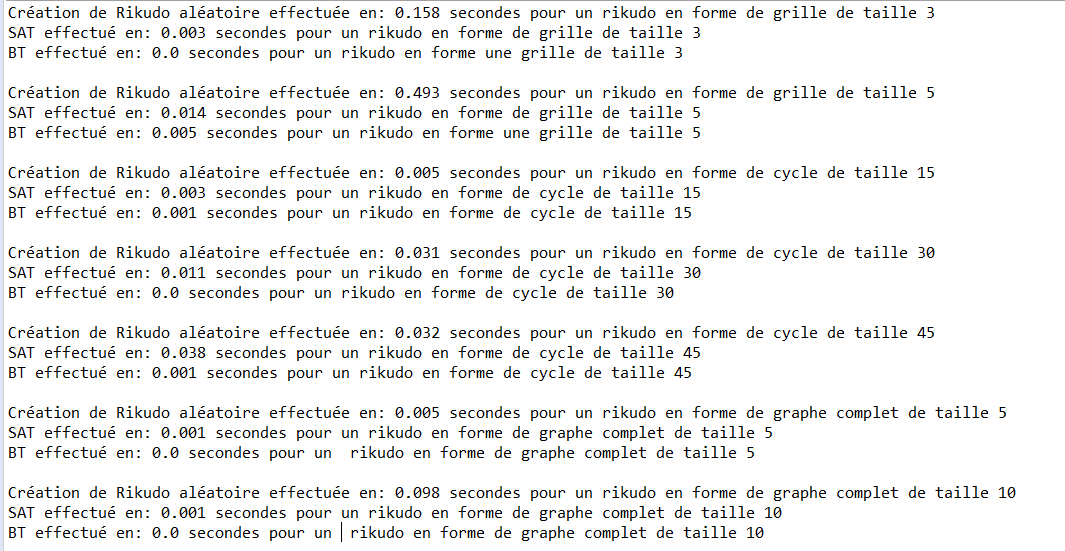
\includegraphics[scale=0.7]{RunTimeRikudo.png}
\end{figure}


\section{Création de puzzles}

Maintenant que nous pouvons résoudre des Rikudos, nous nous intéressons à la conception de tels puzzles. Nous nous intéressons d'abord à la transformation d'un graphe en Rikudo minimal à solution unique, puis nous créons des Rikudos ayant la même forme qu'une image fournie en entrée.

\subsection{À partir d'un graphe}

On utilise l'algorithme $\mathtt{generateRikudo}$ de la classe $\mathtt{Graph}$. Cet algorithme de génération aléatoire de Rikudo à partir de graphe est en deux étapes :

\begin{enumerate}
    \item On commence par rajouter progressivement des contraintes jusqu'à ce qu'il ne reste plus qu'une seule solution.
    \item On enlève les contraintes non essentielles tout en gardant l'unicité de la solution. 
\end{enumerate}

On commence par regarder s'il existe un chemin hamiltonien avec l'algorithme SAT. S'il n'en existe pas, il sera impossible de générer un Rikudo, on renvoie donc une erreur. S'il en existe une on commence à rajouter des contraintes de manière aléatoire. On regarde d'abord si l'on rajoute un diamant ou un label, puis l'on tire aléatoirement un sommet ou une arête parmi les sommets valides afin de rajouter la contrainte. On rajoute la contrainte seulement si on garde au moins une solution, on vérifie cela avec l'algorithme SAT. On utilise ensuite l'algorithme de Backtracking afin de vérifier l'unicité de la solution. 

La deuxième partie correspond à regarder pour chaque contrainte si celle-ci est nécessaire afin de conserver l'unicité de la solution. On procède par essai-erreur. On enlève une contrainte, on regarde avec l'algorithme de Backtracking s'il reste une unique solution. S'il reste une unique solution, alors la contrainte n'était pas nécessaire. Sinon on remet la contrainte. 

\subsection{À partir d'une image}

Notre objectif est maintenant, étant donné une image en noir et blanc, de construire un Rikudo ayant la forme de cette image, et finalement de donner une représentation visuelle sympathique de ce puzzle. On créé donc pour cela un $\mathtt{ImageProcessor}$, en spécifiant la taille que doivent avoir nos tuiles hexagonales à l'affichage, et l'orientation qu'on veut leur donner. On choisit l'image de support et la résolution qu'on veut avoir pour notre puzzle, c'est à dire le nombre de pixels que doit figurer une tuile. On créé ensuite une \textbf{grille hexagonale} recouvrant l'image, représentée par une matrice, et on repère les éléments de cette grille qui doivent faire partie du graphe (éléments correspondant à un pixel noir sur l'image).

On élimine récursivement de cette grille tous les éléments n'ayant que 0 ou 1 voisin, car on veut un graphe connexe et sans impasse. On peut ensuite numéroter les éléments de la grille qu'on a conservé, et créer un $\mathtt{Graph}$ dont ils sont les sommets, et dont les arêtes correspondent aux voisinages dans la grille. On veillera à conserver dans un tableau la position que chaque sommet du graphe occupe dans la grille, cela servira pour la représentation du puzzle.

Puis on utilise la méthode développée à la sous-partie précédente pour transformer ce graphe en Rikudo minimal à solution unique. On utilise finalement l'interface graphique qui nous a été fournie, à laquelle on a ajouté une fonctionnalité pour représenter les numéros des tuiles ($\mathtt{PrintedNumber}$), et quelques figures définies dans $\mathtt{RikudoFigures}$ (hexagones dans leurs deux orientations, diamants dans leur deux orientations) pour représenter le puzzle obtenu, et éventuellement sa solution. On se base pour cela sur la grille définie précédemment.

\begin{figure}[h]
	\centering
	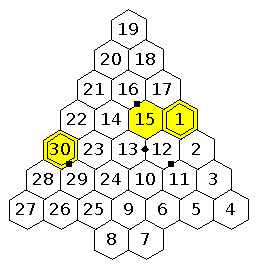
\includegraphics{ChristmasTree.png}
\end{figure}


\section*{Conclusion et perspectives}

Nous avons maintenant une méthode opérationnelle pour générer des Rikudos aux formes sympathiques. Outre les améliorations proposées dans le sujet (ajout de contraintes, interface web...), il pourrait être intéressant de coder une méthode permettant de résoudre un Rikudo à partir d'une image ou d'un scan, pour ne pas avoir à coder "à la main" la représentation du puzzle que l'on cherche à résoudre.
	
\end{document}